\newpage

\subsection{QuizziPedia::Front-End::Models}

	\label{QuizziPedia::Front-End::Models}
	
	\begin{figure}[ht]
		\centering
		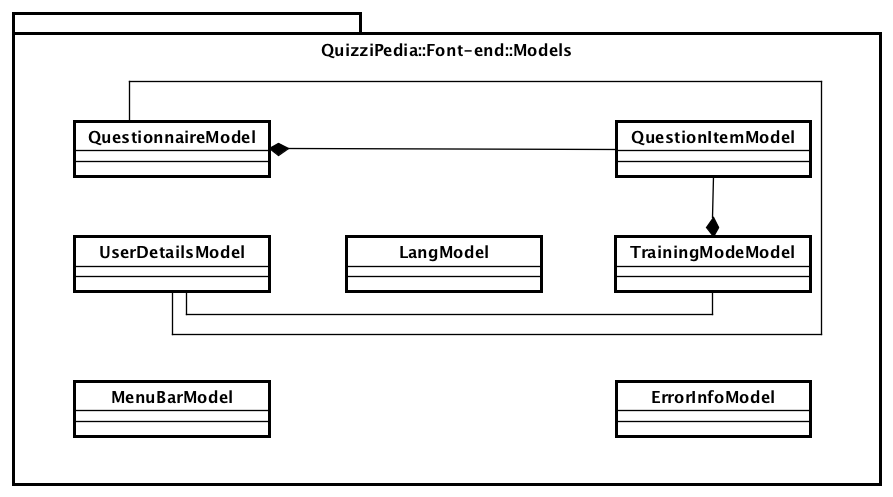
\includegraphics[scale=0.5,keepaspectratio]{UML/Package/QuizziPedia_Front-End_Models.png}
		\caption{QuizziPedia::Front-End::Models}
	\end{figure} \FloatBarrier

	\subsubsection{Informazioni generali}
		\begin{itemize}
			\item \textbf{Descrizione}: package contenente le classi che definiscono la business logic dell'applicazione;
			\item \textbf{Padre}: \texttt{Front-End};
			\item \textbf{Iterazioni con altri componenti}: 
				\begin{itemize}				
					\item \texttt{Controllers}: package contenente i controllers front-end dell'applicazione;
					\item \texttt{Directives}: package contenente le directives front-end dell'applicazione;
					\item \texttt{Models}: package contenente le classi che definiscono la business logic dell'applicazione;
					\item \texttt{Templates}: package contenente i templates necessari per la creazione dinamica delle viste per le domande;
					\item \texttt{Services}: package che contiene le classi individuate che permettono la comunicazione del lato front-end con il lato back-end attraverso l'architettura REST.
				\end{itemize}

		\end{itemize}
	
	\subsubsection{Classi}
		\paragraph{QuizziPedia::Front-End::Models::UserDetailsModel}
		
		\label{QuizziPedia::Front-End::Models:.UserDetailsModel}
		
		\begin{figure}[ht]
			\centering
			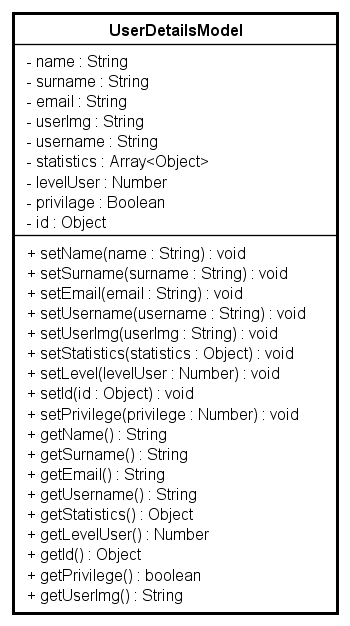
\includegraphics[scale=0.5,keepaspectratio]{UML/Classi/Front-End/QuizziPedia_Front-end_Models_UserDetailsModel.png}
			\caption{QuizziPedia::Front-End::Models::UserDetailsModel}
		\end{figure} \FloatBarrier
		
		\begin{itemize}
			\item \textbf{Descrizione}: rappresenta un utente. Contiene tutte le informazioni necessarie alla presentazione del contenuto di un utente sia nella visualizzazione che nella gestione di un profilo;
			\item \textbf{Utilizzo}: viene utilizzata per memorizzare i dati di un utente;
			\item \textbf{Relazioni con altre classi}: 
			\begin{itemize}
				\item \textit{OUT} \texttt{LoginController}: questa classe permette di gestire l'autenticazione dell'utente al sistema;
				\item \textit{OUT} \texttt{SearchController}: questa classe permette di gestire la ricerca di questionari e utenti all'interno dell'applicazione;
				\item \textit{OUT} \texttt{UserDetailsController}: questa classe permette di gestire i dati di un utente;
				\item \textit{OUT} \texttt{StatisticsController}: questa classe permette di le statistiche di un utente;
			\end{itemize}
			\item \textbf{Attributi}: 
			\begin{itemize}
				\item 
				\texttt{- name: String}\\
				Rappresenta il nome  dell'utente registrato;
				\item 
				\texttt{- surname: String}\\
				Rappresenta il cognome  dell'utente registrato;
				\item 
				\texttt{- email: String}\\
				Rappresenta l'email  dell'utente registrato;
				\item 
				\texttt{- userImg: String}\\
				Rappresenta il path della foto profilo dell'utente registrato;
				\item 
				\texttt{- username: String}\\ 
				Rappresenta l'username con cui viene identificato l'utente all'interno dell'applicazione;		  		
				\item
				\texttt{- statistics: Array Object}\\
				Contenente i seguenti attributi:
				\begin{itemize}
					\item
					\texttt{- topicName: String}\\
					Rappresenta il nome della statistica relativa all'argomento;	 
					\item
					\texttt{- topicLevel: Number}\\
					Identifica il livello di preparazione dell'utente in un determinato argomento;
					\item
					\texttt{- correctAnswers: Number}\\
					Identifica il numero di risposte corrette date dall'utente riguardanti domande di un determinato argomento; 
					\item						
					\texttt{- totalAnswers: Number}\\
					Identifica il numero di risposte totali date dall'utente riguardanti domande di un determinato argomento.		
				\end{itemize}		
				\item 
				\texttt{- levelUser: Number}\\
				Identifica il livello dell'utente;			
				\item 
				\texttt{- privilege: Boolean}\\
				Identifica la tipologia dell'utente;	
				\item
				\texttt{- id: Object}
				Identifica l'\texttt{id} dell'utente;
			\end{itemize}
			\item \textbf{Metodi}: 
			\begin{itemize}
				\item \texttt{+ setName(name: String): void} \\
				Metodo \textit{setter\ped{G}} per il campo dati \texttt{name}.\\
				\textbf{Parametri}:
				\begin{itemize}
					\item {name: String}\\
					Questo parametro contiene il nome dell'utente.
				\end{itemize}
				
				\item \texttt{+ setSurname(surname: String): void} \\
				Metodo \textit{setter\ped{G}} per il campo dati \texttt{surname}.\\
				\textbf{Parametri}:
				\begin{itemize}
					\item {surname: String}\\
					Questo parametro contiene il cognome dell'utente.
				\end{itemize}
				
				\item \texttt{+ setEmail(email: String): void} \\
				Metodo \textit{setter\ped{G}} per il campo dati \texttt{email}.\\
				\textbf{Parametri}:
				\begin{itemize}
					\item {email: String}\\
					Questo parametro contiene l'indirizzo email dell'utente.
				\end{itemize}
				
				\item \texttt{+ setUsername(username: String): void} \\
				Metodo \textit{setter\ped{G}} per il campo dati \texttt{username}.\\
				\textbf{Parametri}:
				\begin{itemize}
					\item {username: String}\\
					Questo parametro contiene lo username dell'utente.
				\end{itemize}
				
				\item \texttt{+ setUserImg(userImg: String): void} \\
				Metodo \textit{setter\ped{G}} per il campo dati \texttt{userImg}.\\
				\textbf{Parametri}:
				\begin{itemize}
					\item {userImg: String}\\
					Questo parametro contiene l'url dell'immagine profilo dell'utente.
				\end{itemize}
				
				\item \texttt{+ setStatistics(statistics: Object): void} \\
				Metodo \textit{setter\ped{G}} per il campo dati \texttt{statistics}.\\
				\textbf{Parametri}:
				\begin{itemize}
					\item {statistics: Object}\\
					Questo parametro contiene le statistiche dell'utente.
				\end{itemize}
				
				\item \texttt{+ setLevel(levelUser: Number): void} \\
				Metodo \textit{setter\ped{G}} per il campo dati \texttt{userLever}.\\
				\textbf{Parametri}:
				\begin{itemize}
					\item {levelUser: Number}\\
					Questo parametro contiene il livello dell'utente.
				\end{itemize}
				
				\item \texttt{+ setId(id: Object): void} \\
				Metodo \textit{setter\ped{G}} per il campo dati \texttt{id}.\\
				\textbf{Parametri}:
				\begin{itemize}
					\item {id: ObjectId}\\
					Questo parametro contiene l'id dell'utente.
				\end{itemize}
				
				\item \texttt{+ setPrivilege(privilege: Number): void} \\
				Metodo \textit{setter\ped{G}} per il campo dati \texttt{privilege}.\\
				\textbf{Parametri}:
				\begin{itemize}
					\item {privilege: Number}\\
					Questo parametro rappresenta la tipologia di utente.
				\end{itemize}
				
				\item \texttt{+ getName(): String} \\
				Metodo \textit{getter\ped{G}} che restituisce il campo dati \texttt{name};
				
				\item \texttt{+ getSurname(): String} \\
				Metodo \textit{getter\ped{G}} che restituisce il campo dati \texttt{surname};
				
				\item \texttt{+ getEmail(): String} \\
				Metodo \textit{getter\ped{G}} che restituisce il campo dati \texttt{email};
				
				\item \texttt{+ getUsername(): String} \\
				Metodo \textit{getter\ped{G}} che restituisce il campo dati \texttt{username};
				
				\item \texttt{+ getStatistics(): Object} \\
				Metodo \textit{getter\ped{G}} che restituisce il campo dati \texttt{statistics};
				
				\item \texttt{+ getLevelUser(): Number} \\
				Metodo \textit{getter\ped{G}} che restituisce il campo dati \texttt{levelUser};
				
				\item \texttt{+ getId(): Object} \\
				Metodo \textit{getter\ped{G}} che restituisce il campo dati \texttt{id};
				
				\item \texttt{+ getPrivilege(): boolean} \\
				Metodo \textit{getter\ped{G}} che restituisce il campo dati \texttt{privilege};
				
				\item \texttt{+ getUserImg(): String} \\
				Metodo \textit{getter\ped{G}} che restituisce il campo dati \texttt{userImg};
				
			\end{itemize}
		\end{itemize}	
		
			
		\paragraph{QuizziPedia::Front-End::Models::TrainingModeModel}
		
		\label{QuizziPedia::Front-End::Models::TrainingModeModel}
		
		\begin{figure}[ht]
			\centering
			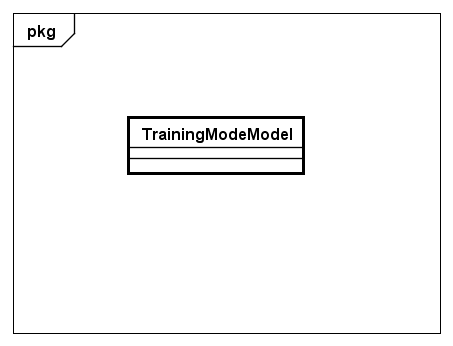
\includegraphics[scale=0.5,keepaspectratio]{UML/Classi/Front-End/QuizziPedia_Front-end_Models_TrainingModeModel.png}
			\caption{QuizziPedia::Front-End::Models::TrainingModeModel}
		\end{figure} \FloatBarrier
		
		\begin{itemize}
			\item \textbf{Descrizione}: rappresenta un allenamento. Contiene tutte le informazioni necessarie alla	presentazione del contenuto di un allenamento;
			\item \textbf{Utilizzo}: viene utilizzata per memorizzare i dati di un allenamento;
			\item \textbf{Relazioni con altre classi}: 
			\begin{itemize}
				\item \textbf{OUT} \texttt{TrainingController}: questa classe permette di gestire la modalità allenamento sottoponendo all'utente le giuste domande adatte al suo livello;
			\end{itemize}
			\item \textbf{Attributi}: 
			\begin{itemize}
				\item \texttt{- argument: String}\\
				Questo attributo rappresenta l'argomento dell'allenamento;
				\item \texttt{- keywords: Array<String>}\\
				Questo attributo rappresenta l'\texttt{array} contenente le parole chiave per l'allenamento;
				\item \texttt{- numberOfQuestions: Number}\\
				Questo attributo rappresenta il numero di domande che l'utente si è prefissato di rispondere per l'allenamento. Se \texttt{-1} allora non esiste un numero di domande impostate, perciò l'allenamento non terminerà fino alla chiusura manuale dell'attività;
				\item \texttt{- questions: Array<QuestionItemModel>}\\
				Questo attributo contiene l'\texttt{array} di \texttt{QuestionItemModel} che rappresenta le domande dell'allenamento fino a quel momento visualizzate, compresa quella visualizzata;
				\item \texttt{- numOfRightAnswer: Number}\\
				Questo attributo rappresenta il numero di domande corrette date;
				\item \texttt{- rightAnswer: Number}\\
				Questo attributo rappresenta le domande corrette a cui si è dato una risposta.
			\end{itemize}
			\item \textbf{Metodi}: 
			\begin{itemize}
				\item \texttt{+ setArgument(argument: String): void} \\
				Metodo \textit{setter\ped{G}} per il campo dati \texttt{argument}.\\
				\textbf{Parametri}:
				\begin{itemize}
					\item {argument: String}\\
					Questo parametro contiene l'argomento dell'allenamento.
				\end{itemize}
				
				\item \texttt{+ setNumberOfQuestions(numberOfQuestions: Number): void} \\
				Metodo \textit{setter\ped{G}} per il campo dati \texttt{numberOfQuestions}.\\
				\textbf{Parametri}:
				\begin{itemize}
					\item {author: ObjectId}\\
					Questo parametro rappresenta l'autore che ha creato la domanda.
				\end{itemize}
				
				\item \texttt{+ getArgument(): String} \\
				Metodo \textit{getter\ped{G}} che restituisce l'argomento dell'allenamento;
				
				\item \texttt{+ getNumeberOfQuestions(): Number} \\
				Metodo \textit{getter\ped{G}} che restituisce il campo dati \texttt{numeberOfQuestions};
				
				\item \texttt{+ addQuestion(question: QuestionItemModel): ObjectId} \\
				Metodo per aggiungere una domanda all'\texttt{array} di domande.\\
				\textbf{Parametri}:
				\begin{itemize}
					\item {question: QuestionItemModel}\\
					Questo parametro rappresenta la domanda da inserire.
				\end{itemize}
				
				\item \texttt{+ removeQuestion(idQuestion: ObjectId): void} \\
				Metodo per poter eliminare una domanda dall'allenamento.\\
				\textbf{Parametri}:
				\begin{itemize}
					\item {idQuestion: ObjectId}\\
					Questo parametro rappresenta l'id della domanda che si vuole rimuove dall'allenamento.
				\end{itemize}
				
				\item \texttt{+ addKeyword(keyword: String): void} \\
				Metodo per aggiungere una parola chiave all'array di parole chiavi.\\
				\textbf{Parametri}:
				\begin{itemize}
					\item {keyword: String}\\
					Questo parametro rappresenta la parola chiave da inserire.
				\end{itemize}
				
				\item \texttt{+ removeKeyword(keyword: String): void} \\
				Metodo per poter eliminare una parola chiave dall'array di parole chiavi.\\
				\textbf{Parametri}:
				\begin{itemize}
					\item {keyword: String}\\
					Questo parametro rappresenta la parola chiave da eliminare.
				\end{itemize}
				
				\item \texttt{+ getResult(): Object} \\
				Metodo \textit{getter\ped{G}} che restituisce risultato fino a quel momento dell'allenamento, ritornando un oggetto contenente il numero di domande giuste e totali.
				
			\end{itemize}
		\end{itemize}
			
			
		\paragraph{QuizziPedia::Front-End::Models::QuestionnaireModel}
		
		\label{QuizziPedia::Front-End::Models::QuestionnaireModel}
		
		\begin{figure}[ht]
			\centering
			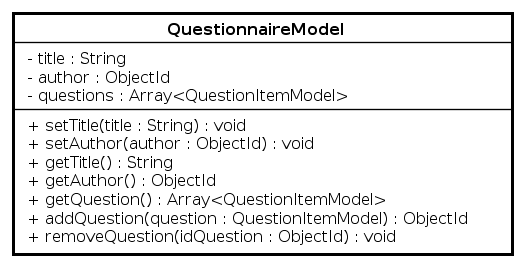
\includegraphics[scale=0.5,keepaspectratio]{UML/Classi/Front-End/QuizziPedia_Front-end_Models_QuestionnaireModel.png}
			\caption{QuizziPedia::Front-End::Models::QuestionnaireModel}
		\end{figure} \FloatBarrier
		
		\begin{itemize}
			\item \textbf{Descrizione}: rappresenta un questionario. Contiene tutte le informazioni necessarie alla presentazione del contenuto del questionario;
			\item \textbf{Utilizzo}: viene utilizzata per memorizzare i dati di un questionario;
			\item \textbf{Relazioni con altre classi}: 
			\begin{itemize}
				\item \textit{IN} \texttt{SearchController}: questa classe permette di gestire la ricerca di questionari e utenti all'interno dell'applicazione;
				\item \textit{IN} \texttt{QuestionnaireDetailsController}: questa classe permette di gestire tutti i questionari creati da un utente; 
				\item \textit{IN} \texttt{FillingQuestionnaireController}: questa classe permette di gestire la creazione e la modifica di una domanda a riempimento di spazi;
				\item \textit{IN} \texttt{CreateQuestionnaireController}: questa classe permette di gestire la creazione di un questionario;
				\item \textit{IN} \texttt{RegistrationManagementController}: questa classe permette di gestire le iscrizione degli utenti ai questionari;
				\item \textit{IN} \texttt{ResultsController}: questa classe permette di gestire i risultati della ricerca effettuata dall'utente.
			\end{itemize}
			\item \textbf{Attributi}: 
			\begin{itemize}
				\item \texttt{- title: String}\\
				Questo attributo rappresenta il titolo del questionario;
				\item \texttt{- author: ObjectId}\\
				Questo attributo rappresenta l'autore del questionario;
				\item \texttt{- questions: Array[QuestionItemModel]}\\
				Questo attributo contiene l'array di \texttt{QuestionItemModel} che rappresenta le domande di un questionario.
			\end{itemize}
			\item \textbf{Metodi}: 
			\begin{itemize}
				\item \texttt{+ setTitle(title: String): void} \\
				Metodo \textit{setter\ped{G}} per il titolo del questionario.\\
				\textbf{Parametri}:
				\begin{itemize}
					\item {title: String}\\
					Questo parametro contiene il titolo del questionario. 
				\end{itemize}
				\item \texttt{+ setAuthor(author: ObjectId): void} \\
				Metodo \textit{setter\ped{G}} per il campo dati \texttt{author}.\\
				\textbf{Parametri}:
				\begin{itemize}
					\item {author: ObjectId}\\
					Questo parametro rappresenta l'autore che ha creato la domanda.
				\end{itemize}
				
				\item \texttt{+ getTitle(): String} \\
				Metodo \textit{getter\ped{G}} che restituisce il titolo del questionario;
				
				\item \texttt{+ getAuthor(): ObjectId} \\
				Metodo \textit{getter\ped{G}} che restituisce il campo dati \texttt{author};
				
				\item \texttt{+ getQuestion(): Array[QuestionItemModel]} \\
				Metodo \textit{getter\ped{G}} che restituisce il campo dati \texttt{questions};
				
				\item \texttt{+ addQuestion(question: QuestionItemModel): ObjectId} \\
				Metodo per aggiungere una domanda all'\texttt{array} di domande.\\
				\textbf{Parametri}:
				\begin{itemize}
					\item {question: QuestionItemModel}\\
					Questo parametro rappresenta la domanda da inserire.
				\end{itemize}
				
				\item \texttt{+ removeQuestion(idQuestion: ObjectId): void} \\
				Metodo per poter eliminare una domanda dal questionario.\\
				\textbf{Parametri}:
				\begin{itemize}
					\item {idQuestion: ObjectId}\\
					Questo parametro rappresenta l'id della domanda che si vuole rimuove dal questionario.
				\end{itemize}
				
				
			\end{itemize}
		\end{itemize}	
		
		
		\paragraph{QuizziPedia::Front-End::Models::QuestionItemModel}
		
		\label{QuizziPedia::Front-End::Models::QuestionItemModel}
		
		\begin{figure}[ht]
			\centering
			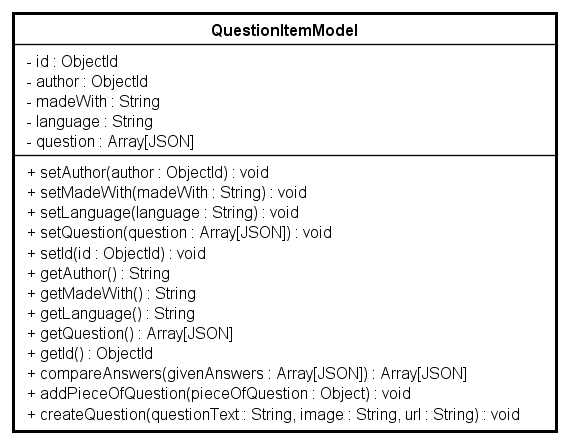
\includegraphics[scale=0.6,keepaspectratio]{UML/Classi/Front-End/QuizziPedia_Front-end_Models_QuestionItemModel.png}
			\caption{QuizziPedia::Front-End::Models::QuestionItemModel}
		\end{figure} \FloatBarrier
		
		\begin{itemize}
			\item \textbf{Descrizione}: rappresenta una domanda. Contiene tutte le informazioni necessarie alla presentazione del contenuto della domanda;
			\item \textbf{Utilizzo}: viene utilizzata per memorizzare i dati di una domanda;
			\item \textbf{Relazioni con altre classi}: 
			\begin{itemize}
				\item \textbf{OUT} \texttt{QuestionsManagementController}: questa classe permette di gestire e di ottenere le domande create dall'utente;
				\item \textbf{OUT} \texttt{TrueFalseQuestionsController}: questa classe permette di gestire la creazione e la modifica di una domanda vero/falso;
				\item \textbf{OUT} \texttt{MultipleQuestionsController}: questa classe permette di gestire la creazione e la modifica di una domanda a risposta multipla; 
				\item \textbf{OUT} \texttt{ConnectionQuestionsController}: questa classe permette di gestire la creazione e la modifica di una domanda a collegamento;
				\item \textbf{OUT} \texttt{ImagesSortingQuestionsController}: questa classe permette di gestire la creazione e la modifica di una domanda a ordinamento immagini;
				\item \textbf{OUT} \texttt{StringsSortingQuestionsController}: questa classe permette di gestire la creazione e la modifica di una domanda a ordinamento di stringhe;
				\item \textbf{OUT} \texttt{FillingQuestionsController}: questa classe permette di gestire la creazione e la modifica di una domanda a riempimento di spazi; 
				\item \textbf{OUT} \texttt{ClickableAreaQuestionsController}: questa classe permette di gestire la creazione e la modifica di una domanda ad area cliccabile;
				\item \textbf{OUT} \texttt{EditorQMLController}: questa classe permette di gestire la creazione e la modifica di domande create tramite editor QML;
				\item \textbf{OUT} \texttt{QuestionsController}: questa classe permette di gestire il recupero delle domande per poterle stampare nella modalità allenamento e nei questionari;
			\end{itemize}
			\item \textbf{Attributi}: 
			\begin{itemize}
				\item \texttt{- id: ObjectId}\\
				Rappresenta l'attributo id della domanda. Viene utilizzato solamente dalle domande recuperate dal database;
				\item \texttt{- author: ObjectId}\\
				Rappresenta il riferimento all'identificativo dell'utente che ha creato la domanda;
				\item \texttt{- madeWith: String}\\ 
				Rappresenta con quale strumento è stata creata la domanda;
				\item \texttt{- language: String}\\
				Rappresenta la lingua in cui è scritta la domanda; 
				\item \texttt{- question: Array<JSON>}\\ 
				Contiene un oggetto di tipo \textit{JSON\ped{G}}. L'oggetto \textit{JSON\ped{G}} è rappresentato dai seguenti campi:
				\begin{itemize}
					\item \texttt{- type: String}\\
					Rappresenta la tipologia di domanda;
					\item \texttt{- questionText: String}\\ 
					Rappresenta il testo della domanda; 
					\item \texttt{- image: String}\\
					Rappresenta l'\textit{URL\ped{G}} dell'immagine associata al testo della domanda; 
					\item \texttt{- answers: Array<JSON>}\\ 
					Contiene un oggetto di tipo \textit{JSON\ped{G}}. L'oggetto \textit{JSON\ped{G}} è rappresentato dai seguenti campi:
					\begin{itemize}	 				  
						\item \texttt{- text: String}\\
						Rappresenta il testo della risposta;
						\item \texttt{- url: String}\\
						Rappresenta l'immagine della risposta;
						\item \texttt{attributesForTForMultiple: Mixed}\\
						Contiene i seguenti attributi:
						\begin{enumerate}
							\item \texttt{- isItRight: Boolean}\\
							Rappresenta se una risposta è giusta o sbagliata.
						\end{enumerate}      
						\item \texttt{- attributesForSorting: Mixed}\\
						Contiene i seguenti attributi:
						\begin{enumerate}
							\item \texttt{- position: Boolean}\\
							Rappresenta quale è la giusta posizione di un testo o immagine all'interno di un esercizio di ordinamento.
						\end{enumerate}  
						\item \texttt{- attributesForLinking: Mixed}\\
						Contiene i seguenti attributi:
						\begin{enumerate}
							\item \texttt{- text1: String}\\
							Rappresenta il primo elemento testuale che deve essere collegato con il secondo elemento testuale o rappresentato da un'immagine;
							\item \texttt{- text2: String}\\
							Rappresenta il secondo elemento testuale che deve essere collegato con il primo elemento testuale o rappresentato da un'immagine;
							\item \texttt{- url1: String}\\
							Rappresenta il primo elemento rappresentato da un'immagine che deve essere collegato con il secondo elemento testuale o rappresentato da un'immagine;
							\item \texttt{- url2: String}\\
							Rappresenta il secondo elemento rappresentato da un'immagine che deve essere collegato con il primo elemento testuale o rappresentato da un immagine.
						\end{enumerate}  
						\item \texttt{- attributesForClickableArea: Mixed}\\
						Contiene i seguenti attributi:
						\begin{enumerate}
							\item \texttt{- x: Number}\\
							Rappresenta la coordinata x di una area cliccabile;  
							\item \texttt{- y: Number}\\
							Rappresenta la coordinata y di una area cliccabile. 
						\end{enumerate}    
						\item \texttt{- attributesForEmptySpaces: Mixed}\\
						Contiene i seguenti attributi:
						\begin{enumerate}
							\item \texttt{- wordNumber: Number}\\
							Rappresenta la posizione dello spazio vuoto in cui deve andare inserita la parola.  
						\end{enumerate}        						  						
					\end{itemize}
				\end{itemize}			
			\end{itemize}
			\item \textbf{Metodi}: 
			\begin{itemize}
				\item \texttt{+ setAuthor(author: ObjectId): void} \\
				Metodo \textit{setter\ped{G}} per il campo dati \texttt{author}.\\
				\textbf{Parametri}:
				\begin{itemize}
					\item {author: ObjectId}\\
					Questo parametro rappresenta l'autore che ha creato la domanda.
				\end{itemize}
				
				\item \texttt{+ setMadeWith(madeWith: String): void} \\
				Metodo \textit{setter\ped{G}} per il campo dati \texttt{madeWith}.\\
				\textbf{Parametri}:
				\begin{itemize}
					\item {madeWith: String}\\
					Questo parametro rappresenta con quale strumento è stata creata la domanda.
				\end{itemize}
				
				\item \texttt{+ setLanguage(language: String): void} \\
				Metodo \textit{setter\ped{G}} per il campo dati \texttt{language}.\\
				\textbf{Parametri}:
				\begin{itemize}
					\item {language: String}\\
					Questo parametro rappresenta la lingua della domanda.
				\end{itemize}
				
				\item \texttt{+ setQuestion(question: Array<JSON>): void} \\
				Metodo \textit{setter\ped{G}} per il campo dati \texttt{question}\\
				\textbf{Parametri}:
				\begin{itemize}
					\item {question: Array<JSON>}\\
					Questo parametro rappresenta l'oggetto \textit{JSON\ped{G}} contenente le parti che compongono la totalità della domanda.
				\end{itemize}
				
				\item \texttt{+ setKeywords(keyword: Array<String>): void} \\
				Metodo \textit{setter\ped{G}} per le keywords della domanda.\\
				\textbf{Parametri}:
				\begin{itemize}
					\item {keyword: Array<String>}\\
					Questo parametro contiene le keywords della domanda. 
				\end{itemize}
				
				\item \texttt{+ getAuthor(): String} \\
				Metodo \textit{getter\ped{G}} per il campo dati \texttt{author};
				
				\item \texttt{+ getMadeWith(): String} \\
				Metodo \textit{getter\ped{G}} per il campo dati \texttt{madeWith};
				
				\item \texttt{+ getLanguage(): String} \\
				Metodo \textit{getter\ped{G}} per il campo dati \texttt{language};

				\item \texttt{+ getQuestion(): Array<JSON>} \\
				Metodo \textit{getter\ped{G}} per il campo dati \texttt{question};
				
				\item \texttt{+ getId(): ObjectId} \\
				Metodo \textit{getter\ped{G}} per il campo dati \texttt{id};
				
				\item \texttt{+ getKeywords(): Array<String>} \\
				Metodo \textit{getter\ped{G}} che restituisce il campo dati \texttt{keywords};
				
				\item \texttt{+ compareAnswers(givenAnswers: Array<JSON>): Array<JSON>} \\
				Metodo che compara le risposte date con quelle corrette. Ritorna un array contenente un valore booleano, che indica se è giusta o meno una domanda, per ogni pezzo di domanda che compone la domanda. \\
				\textbf{Parametri}:
				\begin{itemize}
					\item {givenAnswers: Array<JSON>}\\
					Questo parametro contiene le risposte date dall'utente. 
				\end{itemize}
				
				\item \texttt{+ addPieceOfQuestion(pieceOfQuestion: Object): void} \\
				Metodo che permette di inserire un pezzo di domanda all'attributo \texttt{question}.\\
				\textbf{Parametri}:
				\begin{itemize}
					\item {pieceOfQuestion: Object}\\
					Questo parametro rappresenta un pezzo di domanda.
				\end{itemize}
				
				\item \texttt{+ createQuestion(questionText: String, image: String, url: String):\\ void} \\
				Metodo che inizializza il campo \texttt{question}.\\
				\textbf{Parametri}:
				\begin{itemize}
					\item {questionText: String}\\
					Rappresenta il testo della domanda;
					\item {image: String}\\
					Rappresenta l'\textit{URL\ped{G}} dell'immagine associata al testo della domanda. 
				\end{itemize}	
			\end{itemize}
		\end{itemize}
		
		
		\paragraph{QuizziPedia::Front-End::Models::MenuBarModel}
		
		\label{QuizziPedia::Front-End::Models::MenuBarModel}
		
		\begin{figure}[ht]
			\centering
			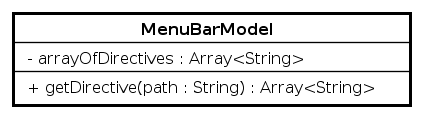
\includegraphics[scale=0.5,keepaspectratio]{UML/Classi/Front-End/QuizziPedia_Front-end_Models_MenuBarModel.png}
			\caption{QuizziPedia::Front-End::Models::MenuBarModel}
		\end{figure} \FloatBarrier
		
		\begin{itemize}
			\item \textbf{Descrizione}: questa classe racchiude i dati necessari per la creazione dinamica della barra menù posizionata in modo fisso su ogni pagina;
			\item \textbf{Utilizzo}: viene utilizzata per memorizzare i dati necessari per la creazione dinamica della barra menù posizionata in modo fisso su ogni pagina;
			\item \textbf{Relazioni con altre classi}: 
			\begin{itemize}
				\item \textbf{IN} \texttt{MenuBarController}: questa classe permette di gestire il menù fisso per ogni pagina;
			\end{itemize}
			\item \textbf{Attributi}: 
			\begin{itemize}
				\item \texttt{- arrayOfDirectives: Array<String>}\\
				Questo attributo contiene l'array di direttive possibili per la creazione dinamica della barra menù posizionata in modo fisso su ogni pagina;
			\end{itemize}
			\begin{itemize}
				\item \texttt{- combination: Array<Number>}\\
				Questo attributo contiene l'array delle combinazioni delle direttive a seconda dell'autore loggato;
			\end{itemize}
			\item \textbf{Metodi}: 
			\begin{itemize}
				\item \texttt{+ getDirective(path: String): Array<String>} \\
				Metodo \textit{getter\ped{G}} che restituisce un array di \texttt{String} contenente le giuste direttive per quella pagina;
			\end{itemize}
		\end{itemize}		
		
		
		
		\paragraph{QuizziPedia::Front-End::Models::LangModel}
		
		\label{QuizziPedia::Front-End::Models::LangModel}
		
		\begin{figure}[ht]
			\centering
			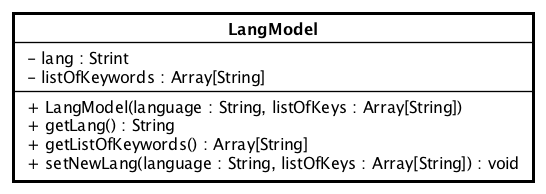
\includegraphics[scale=0.5,keepaspectratio]{UML/Classi/Front-End/QuizziPedia_Front-end_Models_LangModel.png}
			\caption{QuizziPedia::Front-End::Models::LangModel}
		\end{figure} \FloatBarrier
		
		\begin{itemize}
			\item \textbf{Descrizione}: rappresenta le informazioni per la giusta traduzione dell'applicazione;
			\item \textbf{Utilizzo}: viene utilizzata per racchiudere tutte le informazioni riguardanti la giusta traduzione dell'applicazione;
			\item \textbf{Relazioni con altre classi}: 
			\begin{itemize}
				\item \textbf{IN} \texttt{AppRun}: questa classe si preoccupa di creare la prima istanza dell'applicazione.
			\end{itemize}
			\item \textbf{Attributi}: 
			\begin{itemize}
				\item \texttt{- lang: String} \\
				Questo attributo rappresenta la lingua con il quale il sistema verrà visualizzato;  
				\item \texttt{- listOfKeywords: Array<String>} \\
				Questo attributo è un array di String che contiene il set di parole chiave che compongono la struttura dell'applicazione, necessarie per la traduzione delle pagine.
			\end{itemize}
			\item \textbf{Metodi}: 
			\begin{itemize}
				\item \texttt{+ LangModel(language: String, listOfKeys: Array<String>)} \\
				Metodo costruttore della classe.\\
				\textbf{Parametri}:
				\begin{itemize}
					\item {language: String}\\
					Questo parametro rappresenta la lingua con il quale il sistema verrà visualizzato;
					\item {listOfKeys: Array<String>}\\
					Questo parametro è un array di String che contiene il set di parole chiave che compongono la struttura dell'applicazione, necessarie per la traduzione delle pagine. 
				\end{itemize}
				
				\item \texttt{+ getLang(): String} \\
				Metodo che ritorna la lingua del sistema;
				
				\item \texttt{+ getListOfKeywords(): Array<String>} \\
				Metodo che ritorna la lista delle keywords nella lingua corrente del sistema;
				
				\item \texttt{+ setNewLang(language: String, listOfKeys: Array<String>): void} \\
				Metodo che setta la giusta lingua e la lista delle keywords.\\
				\textbf{Parametri}:
				\begin{itemize}
					\item {language: String}\\
					Questo parametro rappresenta la lingua con il quale il sistema verrà visualizzato;
					\item {listOfKeys: Array<String>}\\
					Questo parametro è un array di String che contiene il set di parole chiave che compongono la struttura dell'applicazione, necessarie per la traduzione delle pagine.
				\end{itemize}
				
			\end{itemize}
		\end{itemize}
		
		
		\paragraph{QuizziPedia::Front-End::Models::ErrorInfoModel}
		
		\label{QuizziPedia::Front-End::Models::ErrorInfoModel}
		
		\begin{figure}[ht]
			\centering
			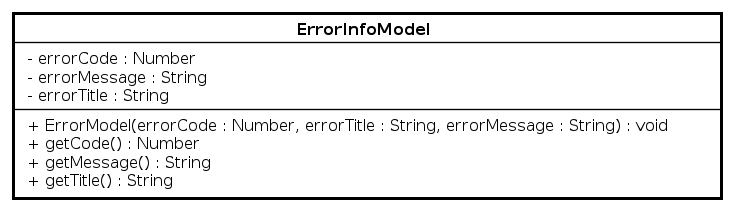
\includegraphics[scale=0.5,keepaspectratio]{UML/Classi/Front-End/QuizziPedia_Front-end_Models_ErrorInfoModel.png}
			\caption{QuizziPedia::Front-End::Models::ErrorInfoModel}
		\end{figure} \FloatBarrier
		
		\begin{itemize}
			\item \textbf{Descrizione}: rappresenta le informazioni di un errore che si è verificato eseguendo una determinata operazione;
			\item \textbf{Utilizzo}: viene utilizzata rappresentare un oggetto di tipo errore;
			\item \textbf{Relazioni con altre classi}: 
			\begin{itemize}
			 	\item \textit{OUT} \texttt{AuthService}: questa classe permette di gestire la registrazione e l'autenticazione di un utente;
			 	\item \textit{OUT} \texttt{SearchService}: questa classe permette di gestire il recupero dei dati dal back-end a seguito di una ricerca effettuata da un utente;
			 	\item \textit{OUT} \texttt{LangService}: questa classe permette di gestire la lingua nella quale si è scelto di utilizzare l'applicazione.
			 	\item \textit{OUT} \texttt{QuizService}: questa classe permette di ottenere i dati di un quiz tramite delle parole chiave inserite dall'utente nella barra di ricerca. Permette inoltre di iscriversi ad un questionario e di scaricare l'intera lista di domande di un questionario a partire dal suo id univoco;
			 	\item \textit{OUT} \texttt{StatisticsService}: questa classe permette di ottenere le statistiche dell'utente;
		 		\item \textit{OUT} \texttt{QuestionsService}: questa classe permette di ottenere domande esistenti e salvare nuove domande;
	 			\item \textit{OUT} \texttt{UserDetailsService}: questa classe permette di ottenere i dati personali degli utenti;
			\end{itemize}
			\item \textbf{Attributi}: 
			\begin{itemize}
				\item \texttt{- errorCode: Number} \\ 
				Rappresenta il codice dell'errore;
				\item \texttt{- errorMessage: String} \\ 
				Rappresenta la descrizione dell'errore; 
				\item \texttt{- errorTitle: String}\\ 
				Rappresenta il titolo del messaggio d'errore.
			\end{itemize}
			\item \textbf{Metodi}
			\begin{itemize}
				\item \texttt{+ ErrorModel(errorCode: Number, errorTitle: String, errorMessage: String) : void} \\
				Metodo costruttore della classe.\\
				\textbf{Parametri}: 
				\begin{itemize}
					\item \texttt{errorCode: Number} \\
					Parametro contenente il codice di errore;
					\item \texttt{errorTitle: String} \\
					Parametro contenente il titolo di errore;
					\item \texttt{errorMessage: String} \\
					Parametro contenente il messaggio di errore.
				\end{itemize}
				\item \texttt{+ getCode() : Number} \\
				Metodo che consente di ottenere il codice dell'errore;
				\item \texttt{+ getMessage() : String} \\
				Metodo che consente di ottenere la descrizione dell'errore;
				\item \texttt{+ getTitle() : String} \\
				Metodo che consente di ottenere il titolo del messaggio d'errore. 
			\end{itemize}
		\end{itemize}
			
											